\chapter{Materiais e Métodos}

\section{Modelo da rede neural DG-CA3}

Baseada principalmente nos modelos de~\cite{kopsickFormation2024,kimAdult2024,yangDynamic2025,chavlisDendrites2017}, a arquitetura
da rede DG-CA3 foi modelada conforme as Figuras~\ref{fig:arquitetura-rede} e~\ref{fig:graph} em escala $\frac{1}{500}$ do
hipocampo do rato, com o número de neurônios por população descritos na Tabela~\ref{tab:neuron_counts}. Os neurônios foram
modelados de forma simples, com um único compartimento, mas com alta fidelidade biológica, utilizando os modelos neuronais e
sinápticos e dados de contagem e conectividade do Hippocampome.org, base de conhecimento de acesso livre que compila diversas
fontes de dados sobre a formação hipocampal~\cite{wheelerHippocampomeorg2023}.

\begin{figure}[H]
    \centering
    \caption{Arquitetura da rede DG-CA3. Sinapses inibitórias são representadas por círculos e excitatórias por flechas.}
    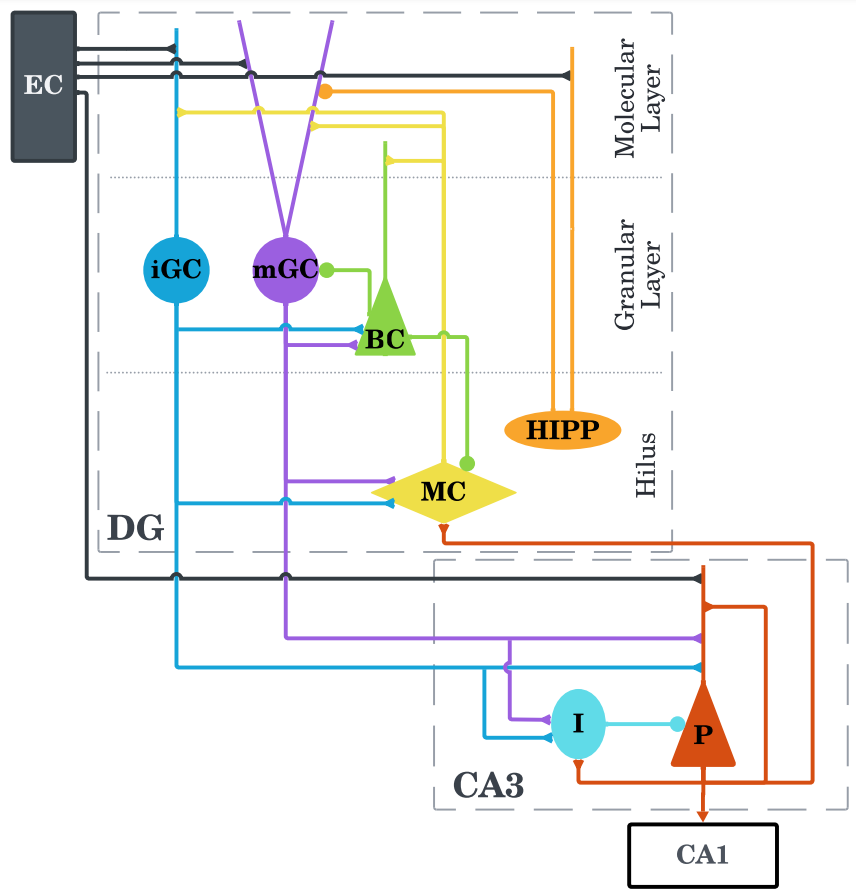
\includegraphics[width=0.87\textwidth]{figuras/arquitetura-rede.png}
    \label{fig:arquitetura-rede}
\end{figure}

\begin{figure}
    \centering
    \caption{Grafo em anel da rede DG-CA3. Cada nó representa um neurônio do modelo, com o mesmo esquema de cores da
    Figura~\ref{fig:arquitetura-rede} para cada neurônio. Cada aresta representa uma sinapse, representada pela cor do neurônio
    pré-sináptico. O EC é representado pelo círculo mais externo em preto, é possível ver a organização lamelar do DG com as mGCs
    e iGCs (vermelho e rosa, respectivamente) e as PCA3s no centro em turquesa. No total, o grafo possui 3.260 nós e 266.596
    arestas.}
    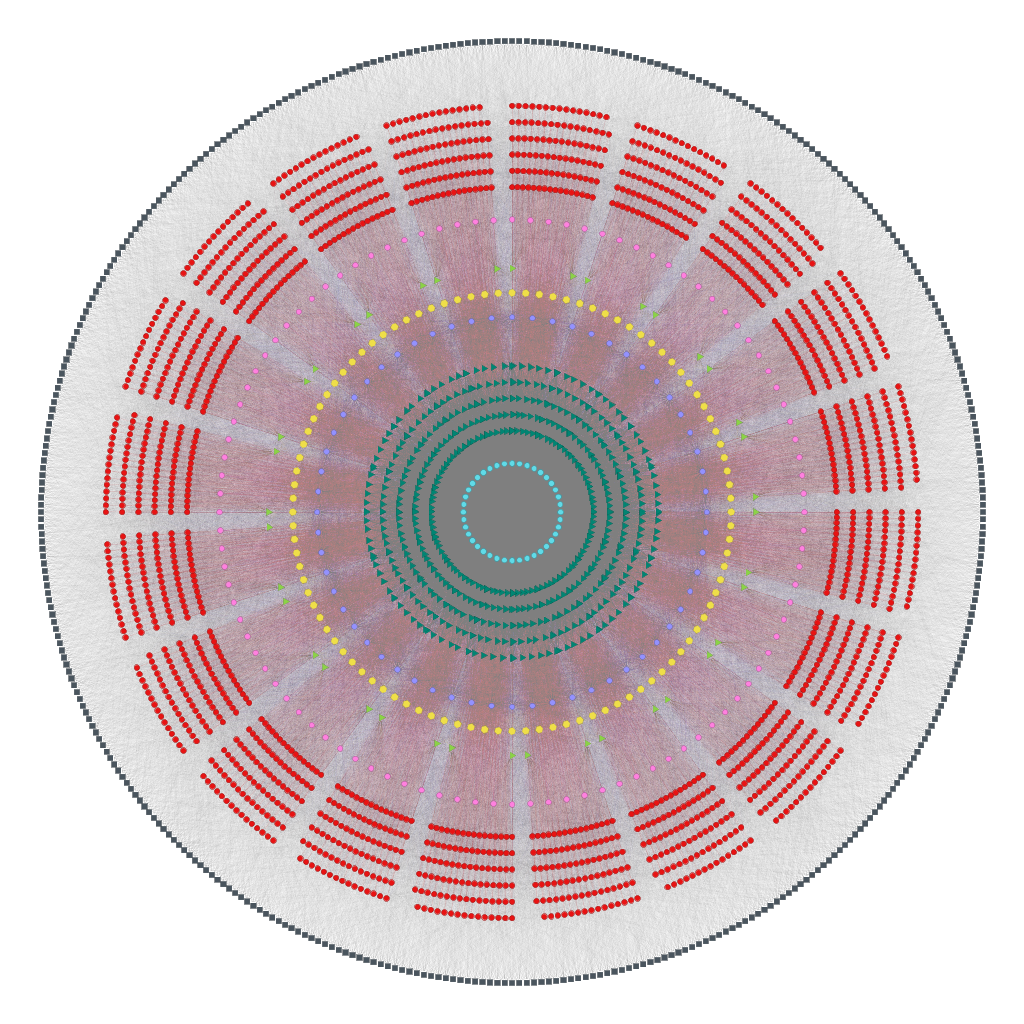
\includegraphics[width=\textwidth]{figuras/network_color_edges}
    \label{fig:graph}
\end{figure}

A entrada da rede é composta pelas células do córtex entorrinal (EC, \textit{Entorhinal Cortex}), com um total de $N_{EC} = 400$
neurônios~\cite{amaralChapter1990,kimAdult2024}. Em cada simulação, o EC como um todo apresenta um padrão específico, onde cada
padrão é representado por uma subpopulação de 10\% de neurônios do EC ativa~\cite{mcnaughtonDead1991}. Os neurônios inativos não
pertencentes ao padrão não disparam durante a simulação, enquanto que os neurônios ativos disparam de acordo com a distribuição de
Poisson com uma taxa de disparo de $\lambda = \SI{40}{\hertz}$. Os neurônios do EC projetam seus axônios através da via perfurante
para neurônios com dendritos na camada molecular do DG: células granulares (GC, \textit{Granule Cells}), células musgosas (MC,
\textit{Mossy Cells})~\cite{scharfmanHilar2013} e células em cesto (BC, \textit{Basket Cells}); bem como para os neurônios do CA3.

As GCs são subdivididas em duas subpopulações: as células granulares maduras (mGC, \textit{mature Granule Cells}) e as células
granulares imaturas (iGC, \textit{immature Granule Cells}), representando as GCs geradas por neurogênese adulta em sua fase
eletrofisiológica característica de 4-6 semanas de idade~\cite{aimoneRegulation2014}. No total, a rede é composta por $N_{GC} =
2000$ GCs ($\frac{1}{500}$ das $10^6$ células granulares do rato)~\cite{westUnbiased1991}, com 5\% delas sendo
iGCs~\cite{cameronAdult2001}, ou seja $N_{mGC} = 1900$ e $N_{iGC} = 100$. Seguindo a organização lamelar do
DG~\cite{sloviterUpdating2012}, as GCs são distribuídas em 20 lamelas, com 100 células por lamela. Cada GC conecta-se com as BCs,
MCs e neurônios do CA3 da mesma lamela, bem como faz conexões excitatórias aleatórias e não lamelares com as células inibitórias
do hilo associadas à via perfurante (HIPP, \textit{HIlar Perforant Path-associated}).

As iGCs, diferentemente das mGCs, possuem características eletrofisiológicas distintas que as tornam mais excitáveis que as mGCs.
Além do mais, para simular a ainda não completa integração no circuito, as iGCs recebem aferências do EC apenas em uma fração
$x_{EC:iGC}$ da probabilidade de conexão entre o EC e as mGCs. O Hippocampome.org~\cite{wheelerHippocampomeorg2023} não fornece as
características das iGCs. Portanto, os parâmetros utilizados para as iGCs foram ajustados a partir dos dados de disparos
de~\citeonline{espositoNeuronal2005} utilizando o método de~\citeonline{nelderSimplex1965}
(Tabela~\ref{tab:izhikevich_neuron_params}).

As BCs ($N_{BC} = 40$) são células inibitórias que garantem a ativação esparsa das GCs através da competição de estilo ``vencedor
leva tudo'' entre elas~\cite{coultripCortical1992,chavlisDendrites2017,kimAdult2024}, onde apenas as GCs mais ativas de uma lamela
se mantêm ativas, inibindo as demais. As HIPPs ($N_{HIPP} = 60$) também contribuem para a esparsidade da ativação das GCs, com uma
inibição mais global, que atua sobre todas as GCs de uma lamela. As MCs ($N_{MC} = 100$) são células excitatórias do hilo que
recebem excitação das GCs e que se projetam para as GCs, BCs e HIPPs através de conexões interlamelares. Por mais que existam
essas projeções excitatórias das MCs para as GCs, seu efeito é, em geral, inibitório através do controle das BCs e
HIPPs~\cite{myersRole2009,scharfmanHilar2013}.

Os parâmetros das HIPPs presentes no Hippocampome.org~\cite{wheelerHippocampomeorg2023} modelam a característica de ``rajada de
disparos de rebote'' (tradução livre do inglês ``\textit{rebound burst firing}''), em que o neurônio apresenta uma rajada de
disparos após o final de um período de hiperpolarização. Esse modelo é incompatível com a rede, pois grandes hiperpolarizações
levam a rajadas de disparos infinitas. Portanto, os parâmetros utilizados para as HIPPs foram retirados
de~\citeonline{modakIzhikevich2018}.

O CA3, diferentemente do DG, não segue uma estrutura lamelar no modelo, já que ele forma uma rede neural muito mais
integrativa~\cite{pakHippocampal2022, watsonHuman2025}. O modelo do CA3 é composto por 600 neurônios piramidais ($N_{PCA3} = 600$)
e 60 neurônios inibitórios ($N_{ICA3} = 60$), modelados de acordo com os dados fisiológicos das células em cesto do
CA3~\cite{wheelerHippocampomeorg2023} de forma a simplificar a variedade de neurônios inibitórios presentes no
CA3~\cite{kopsickFormation2024}. Ambas as populações neuronais recebem aferências do EC e das GCs, com as ICA3s inibindo as PCA3s.
As PCA3s excitam as ICA3s e, importantemente, formam uma rede recorrente ao conectarem-se com outras PCA3s, característica
fundamental para as funções de auto-associação e completamento de padrões do CA3~\cite{kopsickFormation2024, rollsMechanisms2013}.
As PCA3s também enviam retroprojeções para o DG, conectando-se com as MCs no modelo, processo que contribui para a separação de
padrões~\cite{myersPattern2011}.

Todas as simulações foram realizadas com o Brian2~\cite{stimbergBrian2019a}, utilizando o método de Runge-Kutta de 4ª ordem com
passo de tempo fixo de \SI{0.1}{\milli\second}~\cite{butcherHistory1996}. Os parâmetros dos neurônios e suas sinapses podem ser
encontrados nas Tabelas~\ref{tab:izhikevich_neuron_params} e~\ref{tab:synapse_params}, respectivamente. A duração de uma única
simulação para um padrão de entrada é de \SI{500}{\milli\second} para que a rede alcance um estado de equilíbrio, com a fase de
gravação de padrões ocorrendo em seguida por \SI{1000}{\milli\second}. As conexões sinápticas são mantidas fixas entre todas as
simulações.

% Neuron Counts Table
% Required packages: \usepackage{amsmath}, \usepackage{graphicx}
\begin{table}[h!]
\centering
\renewcommand{\arraystretch}{1.4}
\begin{tabular}{lc}
\toprule
\textbf{Célula} & \textbf{N} \\
\midrule
$\vcenter{\hbox{
\includegraphics[height=1.5em]{figuras/neurônios/pp.png}}}$ Córtex Entorrinal & 400 \\
$\vcenter{\hbox{
\includegraphics[height=1.5em]{figuras/neurônios/mgc.png}}}$ Granular madura & 1900 \\
$\vcenter{\hbox{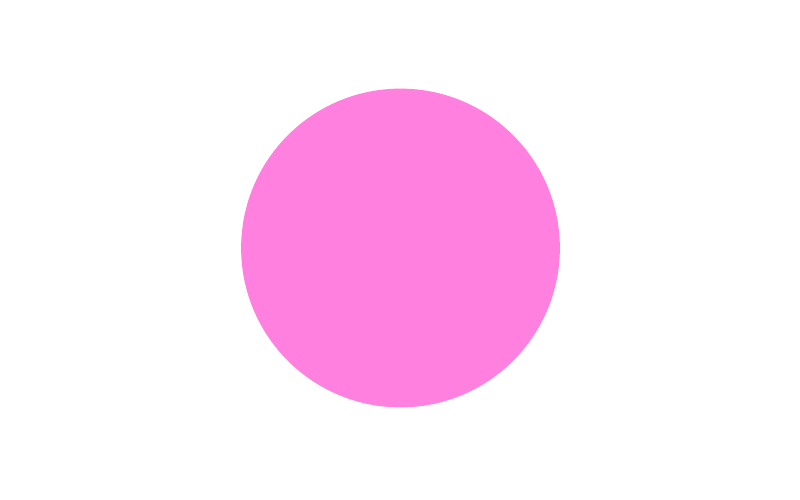
\includegraphics[height=1.5em]{figuras/neurônios/igc.png}}}$ Granular imatura & 100 \\
$\vcenter{\hbox{
\includegraphics[height=1.5em]{figuras/neurônios/mc.png}}}$ Musgosa & 100 \\
$\vcenter{\hbox{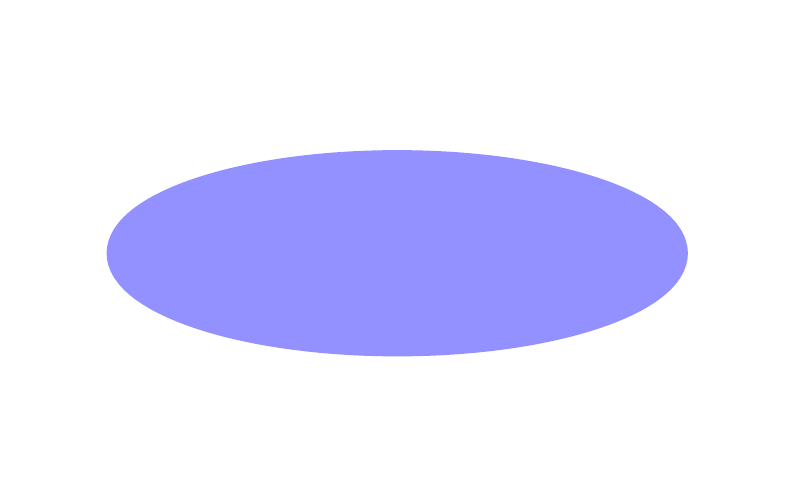
\includegraphics[height=1.5em]{figuras/neurônios/hipp.png}}}$ HIPP & 60 \\
$\vcenter{\hbox{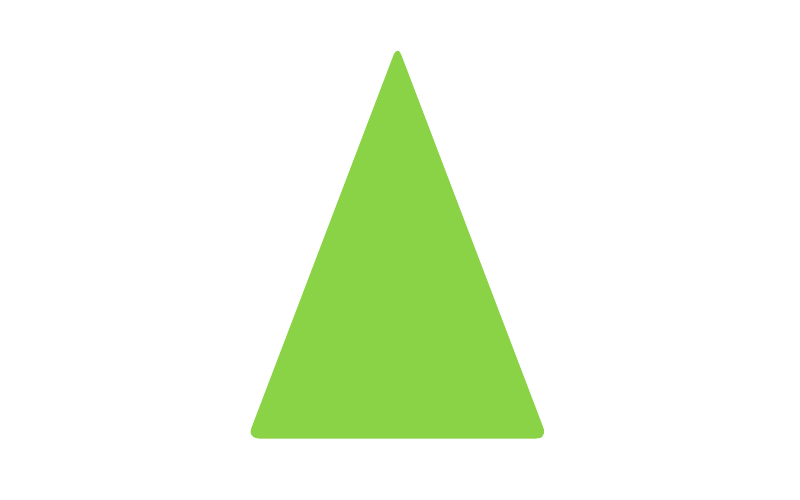
\includegraphics[height=1.5em]{figuras/neurônios/bc.png}}}$ Em cesto & 40 \\
$\vcenter{\hbox{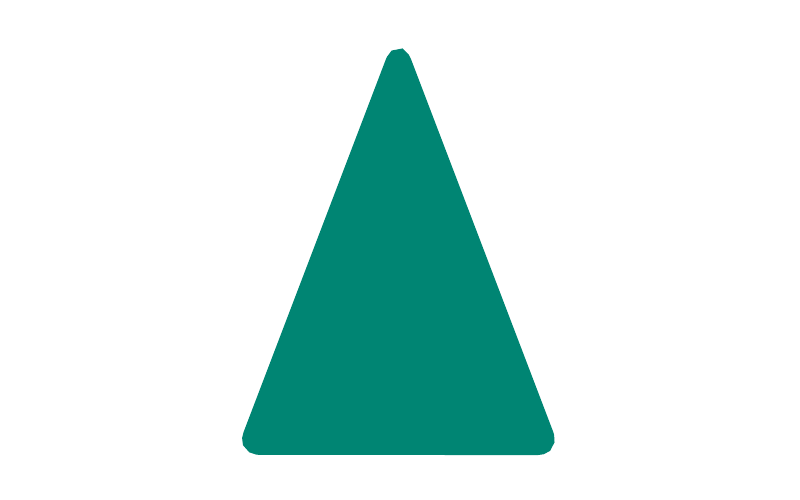
\includegraphics[height=1.5em]{figuras/neurônios/pca3.png}}}$ Piramidal do CA3 & 600 \\
$\vcenter{\hbox{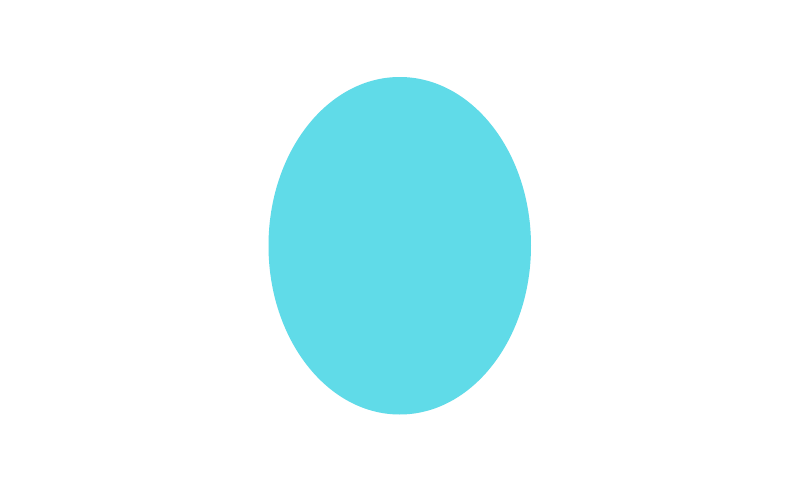
\includegraphics[height=1.5em]{figuras/neurônios/ica3.png}}}$ Inibitória do CA3 & 60 \\
\bottomrule
\end{tabular}
\caption{Quantidade de neurônios por população (N).}\label{tab:neuron_counts}
\end{table}


\section{Modelo de neurônio}

Os neurônios foram modelados de acordo com o modelo de neurônio de Izhikevich de 9
parâmetros~\cite[cap.~8]{izhikevichDynamical2006} e um único compartimento, sem considerar dendritos ou axônios. Esse modelo foi
escolhido neste trabalho e por~\citeonline{wheelerHippocampomeorg2023} por ser capaz de capturar o comportamento dinâmico de
neurônios em uma ampla variedade de condições com plausibilidade biológica, como o modelo de
Hodgkin-Huxley~\cite{hodgkinQuantitative1952b}, ao mesmo tempo em que apresenta um modelo matemático mais simples e
computacionalmente mais eficiente. O modelo de neurônio de Izhikevich é descrito pelas seguintes equações:


\begin{equation}
\label{eq_izhikevich_1}
C_m \frac{dV_m}{dt} = k (V_m - V_r)(V_m - V_t) - u + I
\end{equation}

\begin{equation}
\label{eq_izhikevich_2}
\frac{du}{dt} = a [b(V_m-V_r) - u]
\end{equation}

Onde $V_m$ é o potencial de membrana, $u$ é a variável de recuperação, $C_m$ é a capacitância da membrana, $V_r$ é o
potencial de repouso, $V_t$ é o potencial de limiar, $I$ é a corrente total que flui para o neurônio e $k$, $a$ e $b$ são
constantes que definem as características dinâmicas do neurônio. Além das equações diferenciais acima, que definem a evolução
temporal do potencial de membrana e da variável de recuperação, o modelo de neurônio de Izhikevich também inclui uma regra para
a geração de potenciais de ação, definida pela equação~\ref{eq_izhikevich_3}.

\begin{equation}
\label{eq_izhikevich_3}
\text{se } V_m \geq V_{\text{peak}}, \quad
\begin{cases}
V_m \gets V_{min} \\
u \gets u + d
\end{cases}
\end{equation}

Quando o potencial de membrana atinge o valor de pico $V_{\text{peak}}$, um potencial de ação é gerado e o potencial de membrana é
redefinido para o potencial pós-disparo $V_{min}$ e a variável de recuperação $u$ é incrementada em $d$, dificultando a geração de
um próximo potencial de ação.

% Required packages: \usepackage{amsmath}, \usepackage{graphicx}, \usepackage{multirow}
\begin{table}[h!]
\centering
\renewcommand{\arraystretch}{1.4}
\resizebox{\textwidth}{!}{%
\begin{tabular}{lccccccccc}
\toprule
\multirow{2}{*}{\textbf{Célula}} & \textbf{$k$} & \textbf{$a$} & \textbf{$b$} & \textbf{$d$} & \textbf{$C_m$} & \textbf{$V_r$} & \textbf{$V_t$} & \textbf{$V_{min}$} & \textbf{$V_{peak}$} \\
 & (nS/mV) & (ms$^{-1}$) & (nS) & (pA) & (pF) & (mV) & (mV) & (mV) & (mV) \\
\midrule
$\vcenter{\hbox{
\includegraphics[height=1.5em]{figuras/neurônios/mgc.png}}}$ Granular madura & 0.45 & 0.003 & 24.48 & 50 & 38 & -77.4 & -44.9 & -66.47 & 15.49 \\
$\vcenter{\hbox{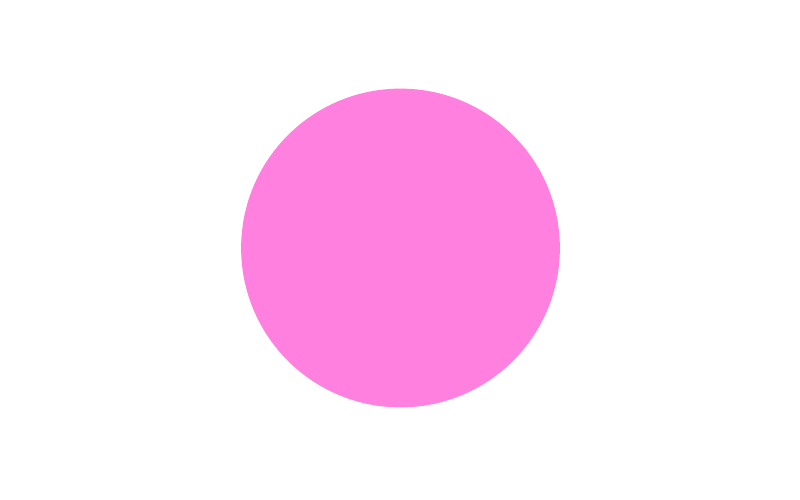
\includegraphics[height=1.5em]{figuras/neurônios/igc.png}}}$ Granular imatura & 0.139 & 0.002 & -1.877 & 12.149 & 24.6 & -63.66 & -38.41 & -48.2 & 83.5 \\
$\vcenter{\hbox{
\includegraphics[height=1.5em]{figuras/neurônios/mc.png}}}$ Musgosa & 1.5 & 0.004 & -20.84 & 117 & 258 & -63.67 & -37.11 & -47.98 & 28.29 \\
$\vcenter{\hbox{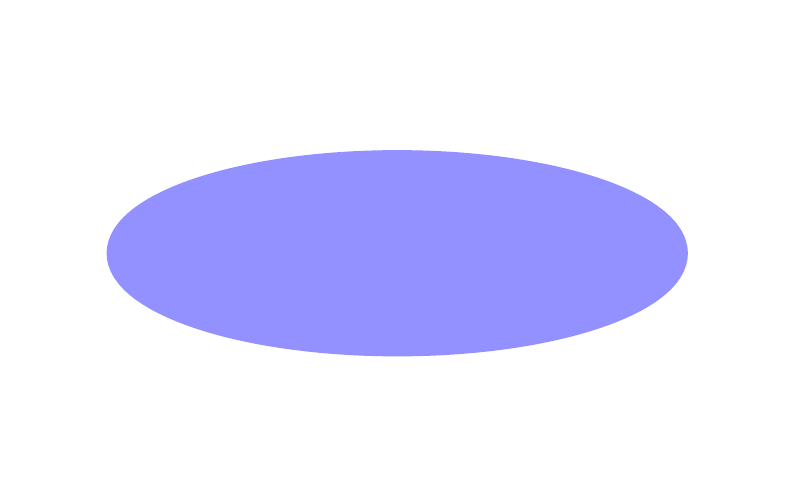
\includegraphics[height=1.5em]{figuras/neurônios/hipp.png}}}$ HIPP & 0.01 & 0.004 & -2 & 40.52 & 58.7 & -70 & -50 & -75 & 90 \\
$\vcenter{\hbox{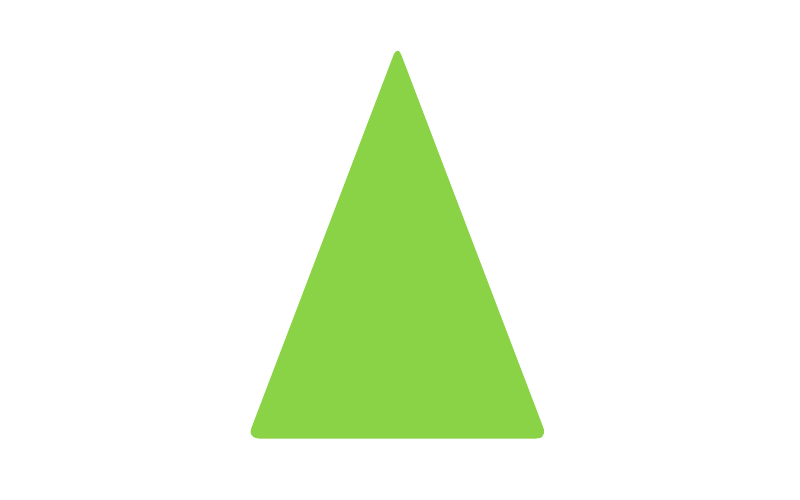
\includegraphics[height=1.5em]{figuras/neurônios/bc.png}}}$ Em cesto & 0.81 & 0.097 & 1.89 & 553 & 208 & -61.02 & -37.84 & -36.23 & 14.08 \\
$\vcenter{\hbox{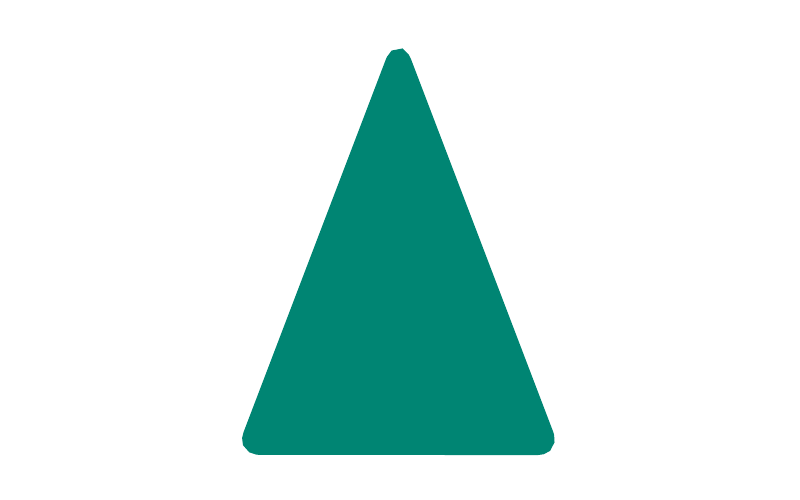
\includegraphics[height=1.5em]{figuras/neurônios/pca3.png}}}$ Piramidal do CA3 & 0.79 & 0.008 & -42.55 & 588 & 366 & -63.2 & -33.6 & -38.87 & 35.86 \\
$\vcenter{\hbox{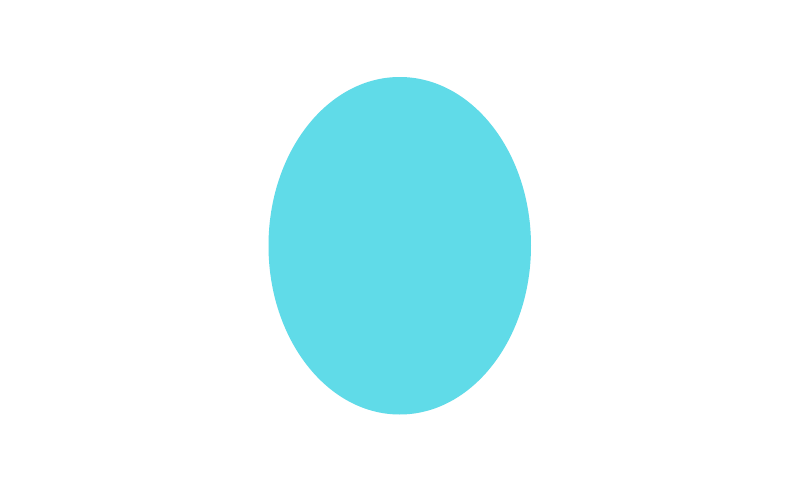
\includegraphics[height=1.5em]{figuras/neurônios/ica3.png}}}$ Inibitória do CA3 & 1 & 0.004 & 9.26 & -6 & 45 & -57.51 & -23.38 & -47.56 & 18.45 \\
\bottomrule
\end{tabular}}
\caption{Parâmetros do modelo Izhikevich por tipo de neurônio.}\label{tab:izhikevich_neuron_params}
\end{table}


\section{Modelo de sinapse}

O modelo de sinapse, assim como o de neurônio, foi definido a partir do Hippocampome.org~\cite{wheelerHippocampomeorg2023},
seguindo a formulação de~\citeonline{sennAlgorithm2001,mongilloSynaptic2008a}. Esse modelo modela a plasticidade de curto prazo,
seja ela depressão de curto prazo, causada pela depleção de neurotransmissores, ou potenciação de curto prazo, causada pelo
acúmulo de cálcio, ambas na escala dos décimos de segundos. Cada sinapse possui 5 parâmetros (descritos na
Tabela~\ref{tab:synapse_params}): a condutância máxima da sinapse no caso de nenhuma depleção de recursos sinápticos $g$, a
proporção de recursos utilizados a cada disparo $U_{se}$, a constante de tempo de decaimento da corrente sináptica $\tau_d$, a
constante de tempo de facilitação $\tau_f$, e a constante de tempo de recuperação dos recursos
$\tau_r$~\cite{moradiNormalized2022}. Outro parâmetro apresentado na Tabela~\ref{tab:synapse_params} é a probabilidade de conexão
$P$. Por mais que o Hippocampome.org possua dados das probabilidades de conexão entre as populações neuronais \textit{in vivo},
pela escala reduzida da rede, foi necessário aumentá-la de forma a que haja atividade na rede enquanto a atividade esparsa fosse
mantida.

O modelo é descrito por três variáveis de estado: a utilização dos recursos sinápticos ($U$), a recuperação desses recursos ($R$)
e a porcentagem de recursos em estado ativo ($A$). Inicialmente, $U_{t_0} = 0$, $R_{t_0} = 1$ e $A_{t_0} = 0$, 
visto que todos os recursos estão disponíveis para ser utilizados. A evolução temporal dessas
variáveis é governada pelo seguinte sistema de equações diferenciais:

\begin{equation}
    \label{eq_tsodyks_dU}
    \frac{dU}{dt} = \frac{-U}{\tau_f} + U_{se}(1-U_{-}) \delta(\Delta t_i)
\end{equation}

\begin{equation}
    \label{eq_tsodyks_dR}
    \frac{dR}{dt} = \frac{1-R-A}{\tau_r} - U_{+} R_{-} \delta(\Delta t_i)
\end{equation}

\begin{equation}
    \label{eq_tsodyks_dA}
    \frac{dA}{dt} = \frac{-A}{\tau_d} + U_{+} R_{-} \delta(\Delta t_i)
\end{equation}

nde $\delta$ é a função delta de Dirac, que resulta em 1 apenas quando $\Delta t_i = t - t_i = 0$, ou seja, apenas no tempo $t$
correspondente ao tempo do evento sináptico $t_i$. $U_{+}$ corresponde ao valor de $U$ logo após o evento sináptico, enquanto que
$R_{-}$ corresponde ao valor de $R$ logo antes do mesmo.

A partir dessas equações, a corrente sináptica é dada por:

\begin{equation}
    \label{eq_tsodyks_I}
    I = k \cdot A \cdot g \cdot (V_m - E)
\end{equation}

onde $V_m$ é o potencial de membrana do neurônio pós-sináptico, $E$ é o potencial de reversão da sinapse, para sinapses
inibitórias e excitatórias, respectivamente, $E_{inh} = \SI{-86}{\milli\volt}$ e $E_{exc} = \SI{0}{\milli\volt}$, e $k$
é uma constante de escala definida como $k = 10$ para todas as sinapses. Essa constante de escala é necessária por conta
da escala reduzida da rede, visto que, pelo baixo número de sinapses do modelo comparado ao hipocampo do rato, sem o 
escalamento a rede toda ficaria silenciosa.


% Synapse Parameters Table
% Required packages: \usepackage{amsmath}, \usepackage{graphicx}, \usepackage{multirow}
\begin{table}[h!]
\centering
\renewcommand{\arraystretch}{1.4}
\resizebox{\textwidth}{!}{%
\begin{tabular}{llccccccc}
\toprule
\multirow{2}{*}{\textbf{Pré-sináptico}} & \multirow{2}{*}{\textbf{Pós-sináptico}} & \multirow{2}{*}{\textbf{Conexão}} & $P$ & \textbf{$g$} & \textbf{$\tau_d$} & \textbf{$\tau_r$} & \textbf{$\tau_f$} & \textbf{$U$} \\
 & & & (\%) & (nS) & (ms) & (ms) & (ms) &  \\
\midrule
$\vcenter{\hbox{
\includegraphics[height=1.5em]{figuras/neurônios/pp.png}}}$ Córtex Entorrinal & $\vcenter{\hbox{
\includegraphics[height=1.5em]{figuras/neurônios/mgc.png}}}$ Granular madura & Aleatória & 8 & 1.825 & 5.333 & 266.239 & 18.714 & 0.27 \\
$\vcenter{\hbox{
\includegraphics[height=1.5em]{figuras/neurônios/pp.png}}}$ Córtex Entorrinal & $\vcenter{\hbox{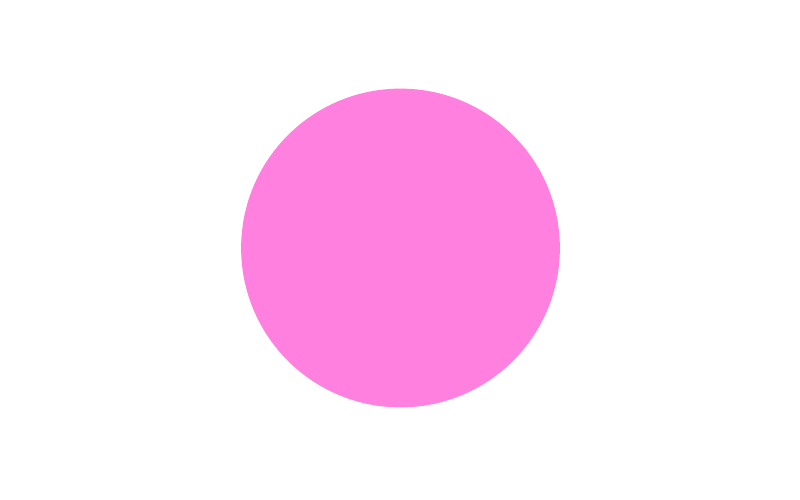
\includegraphics[height=1.5em]{figuras/neurônios/igc.png}}}$ Granular imatura & Aleatória & 8 & 1.825 & 5.333 & 266.239 & 18.714 & 0.27 \\
$\vcenter{\hbox{
\includegraphics[height=1.5em]{figuras/neurônios/pp.png}}}$ Córtex Entorrinal & $\vcenter{\hbox{
\includegraphics[height=1.5em]{figuras/neurônios/mc.png}}}$ Musgosa & Aleatória & 20 & 1.422 & 4.671 & 319.835 & 57.766 & 0.204 \\
$\vcenter{\hbox{
\includegraphics[height=1.5em]{figuras/neurônios/pp.png}}}$ Córtex Entorrinal & $\vcenter{\hbox{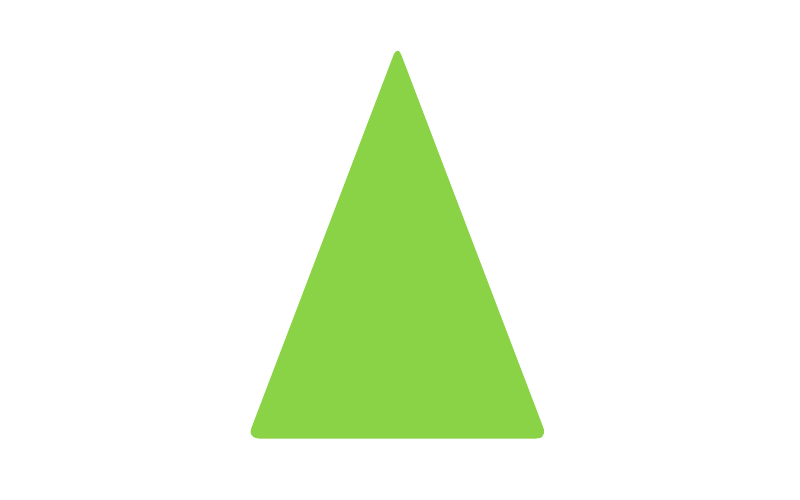
\includegraphics[height=1.5em]{figuras/neurônios/bc.png}}}$ Em cesto & Aleatória & 20 & 1.406 & 3.849 & 144.415 & 48.2 & 0.214 \\
$\vcenter{\hbox{
\includegraphics[height=1.5em]{figuras/neurônios/pp.png}}}$ Córtex Entorrinal & $\vcenter{\hbox{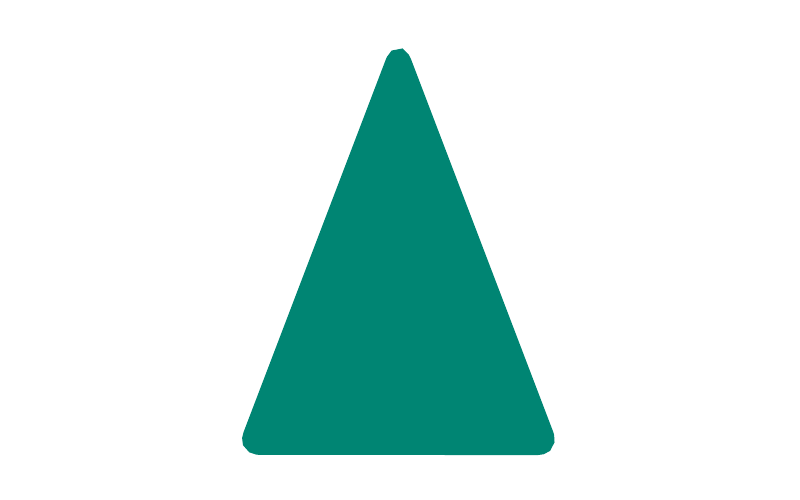
\includegraphics[height=1.5em]{figuras/neurônios/pca3.png}}}$ Piramidal do CA3 & Aleatória & 4 & 1.065 & 6.55 & 258.318 & 53.478 & 0.184 \\
$\vcenter{\hbox{
\includegraphics[height=1.5em]{figuras/neurônios/pp.png}}}$ Córtex Entorrinal & $\vcenter{\hbox{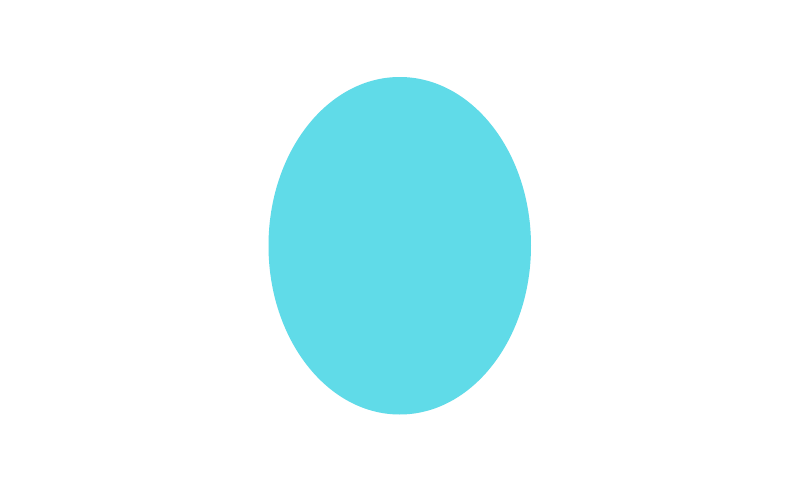
\includegraphics[height=1.5em]{figuras/neurônios/ica3.png}}}$ Inibitória do CA3 & Aleatória & 20 & 1.556 & 3.602 & 457.468 & 35.904 & 0.21 \\
$\vcenter{\hbox{
\includegraphics[height=1.5em]{figuras/neurônios/mgc.png}}}$ Granular madura & $\vcenter{\hbox{
\includegraphics[height=1.5em]{figuras/neurônios/mc.png}}}$ Musgosa & Lamelar & 20 & 1.713 & 5.347 & 428.583 & 73.479 & 0.151 \\
$\vcenter{\hbox{
\includegraphics[height=1.5em]{figuras/neurônios/mgc.png}}}$ Granular madura & $\vcenter{\hbox{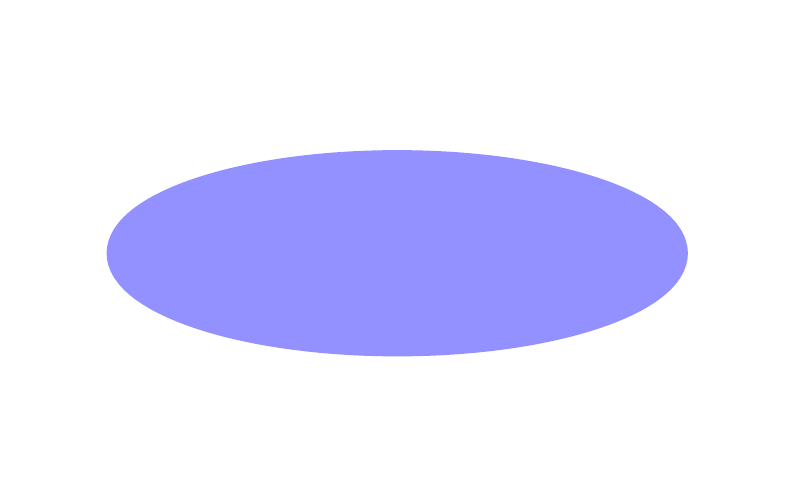
\includegraphics[height=1.5em]{figuras/neurônios/hipp.png}}}$ HIPP & Aleatória & 5 & 1.305 & 5.181 & 462.814 & 48.986 & 0.15 \\
$\vcenter{\hbox{
\includegraphics[height=1.5em]{figuras/neurônios/mgc.png}}}$ Granular madura & $\vcenter{\hbox{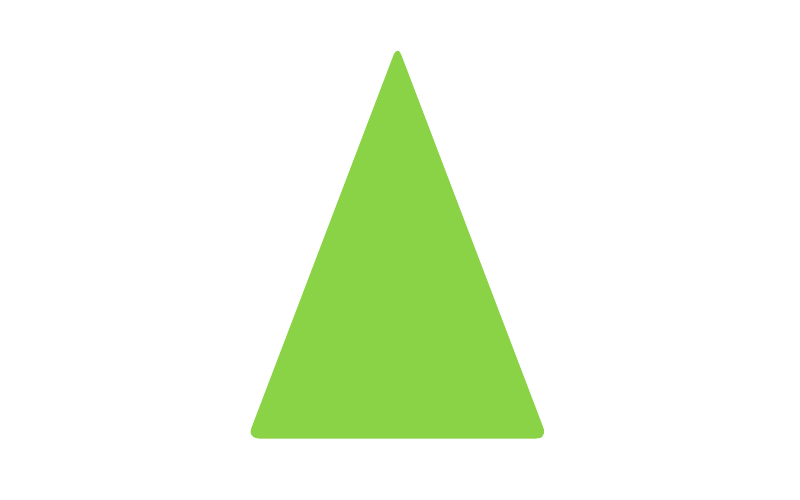
\includegraphics[height=1.5em]{figuras/neurônios/bc.png}}}$ Em cesto & Lamelar & 100 & 1.458 & 3.566 & 151.265 & 62.278 & 0.197 \\
$\vcenter{\hbox{
\includegraphics[height=1.5em]{figuras/neurônios/mgc.png}}}$ Granular madura & $\vcenter{\hbox{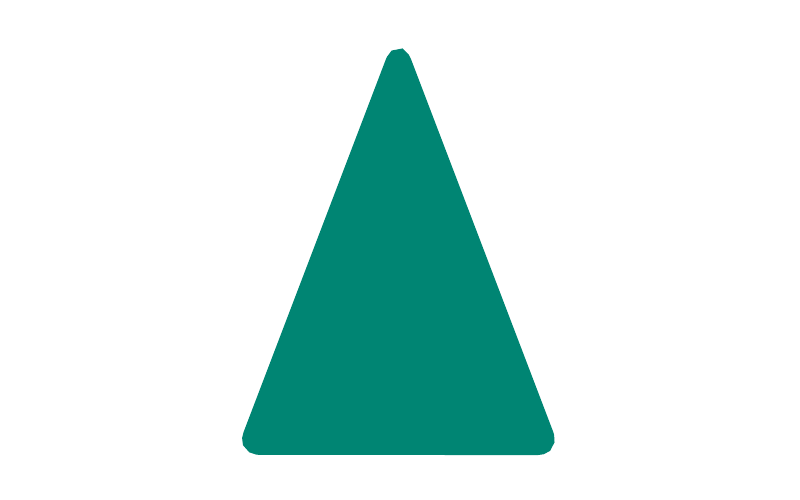
\includegraphics[height=1.5em]{figuras/neurônios/pca3.png}}}$ Piramidal do CA3 & Lamelar & 60 & 1.384 & 6.657 & 278.286 & 78.584 & 0.155 \\
$\vcenter{\hbox{
\includegraphics[height=1.5em]{figuras/neurônios/mgc.png}}}$ Granular madura & $\vcenter{\hbox{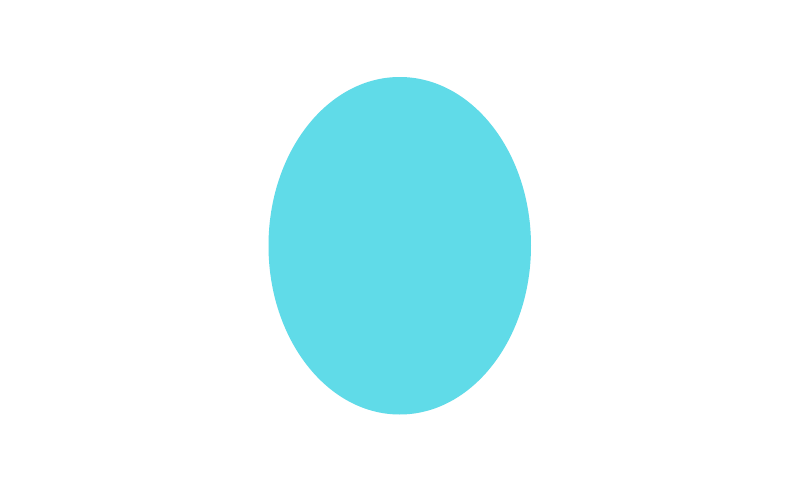
\includegraphics[height=1.5em]{figuras/neurônios/ica3.png}}}$ Inibitória do CA3 & Lamelar & 100 & 1.625 & 3.915 & 518.934 & 43.274 & 0.176 \\
$\vcenter{\hbox{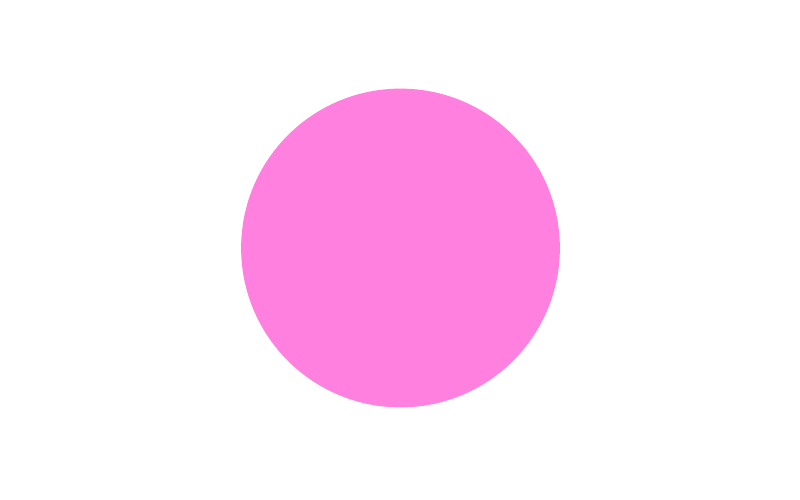
\includegraphics[height=1.5em]{figuras/neurônios/igc.png}}}$ Granular imatura & $\vcenter{\hbox{
\includegraphics[height=1.5em]{figuras/neurônios/mc.png}}}$ Musgosa & Lamelar & 20 & 1.713 & 5.347 & 428.583 & 73.479 & 0.151 \\
$\vcenter{\hbox{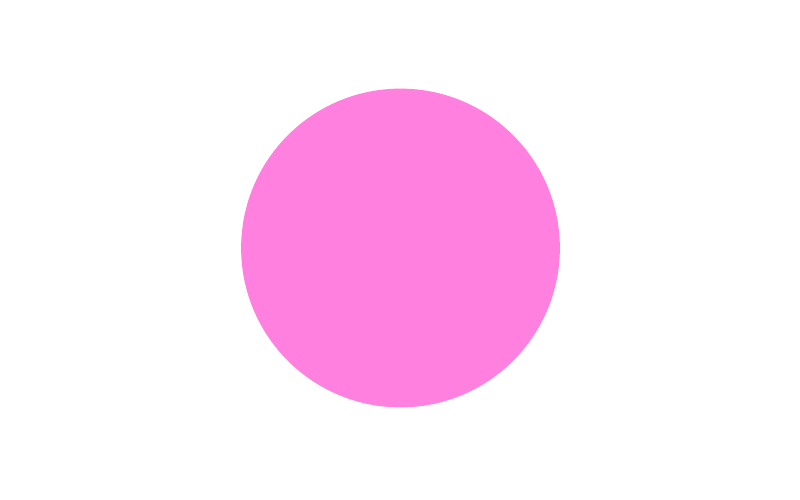
\includegraphics[height=1.5em]{figuras/neurônios/igc.png}}}$ Granular imatura & $\vcenter{\hbox{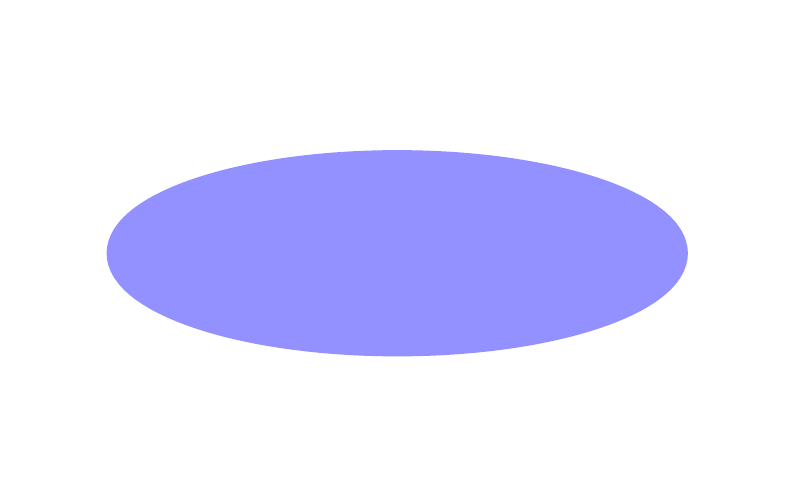
\includegraphics[height=1.5em]{figuras/neurônios/hipp.png}}}$ HIPP & Aleatória & 5 & 1.305 & 5.181 & 462.814 & 48.986 & 0.15 \\
$\vcenter{\hbox{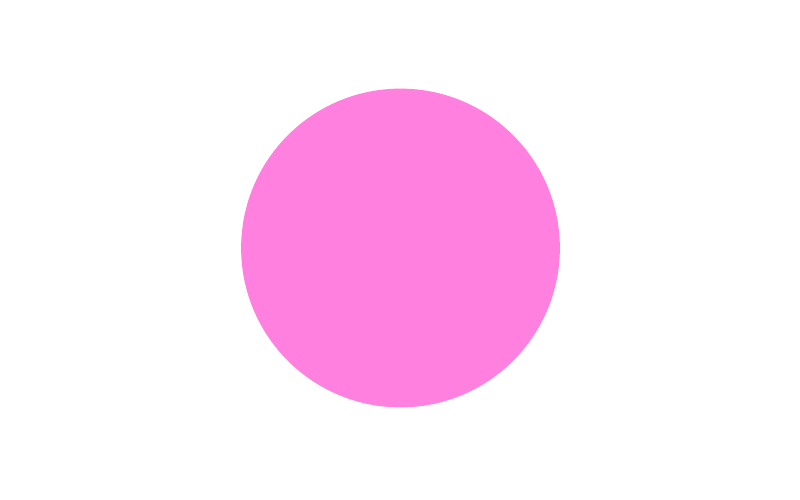
\includegraphics[height=1.5em]{figuras/neurônios/igc.png}}}$ Granular imatura & $\vcenter{\hbox{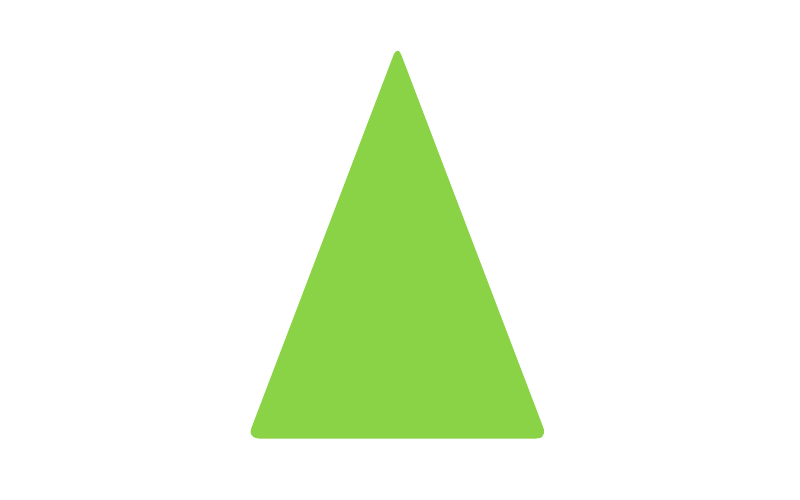
\includegraphics[height=1.5em]{figuras/neurônios/bc.png}}}$ Em cesto & Lamelar & 100 & 1.458 & 3.566 & 151.265 & 62.278 & 0.197 \\
$\vcenter{\hbox{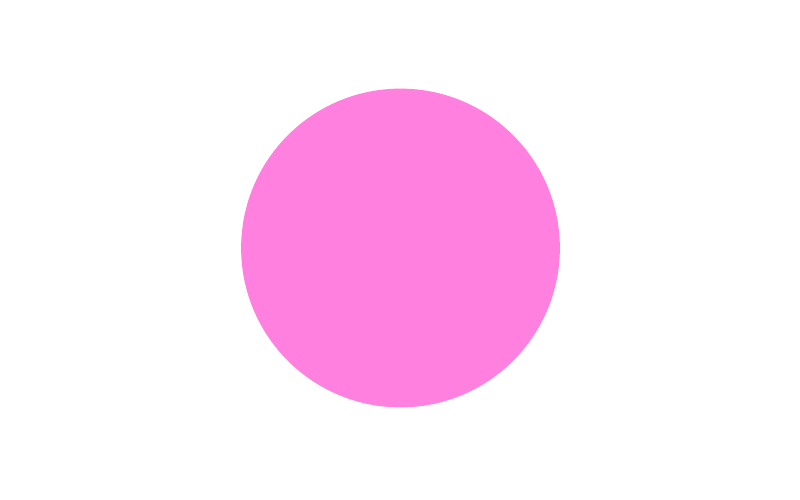
\includegraphics[height=1.5em]{figuras/neurônios/igc.png}}}$ Granular imatura & $\vcenter{\hbox{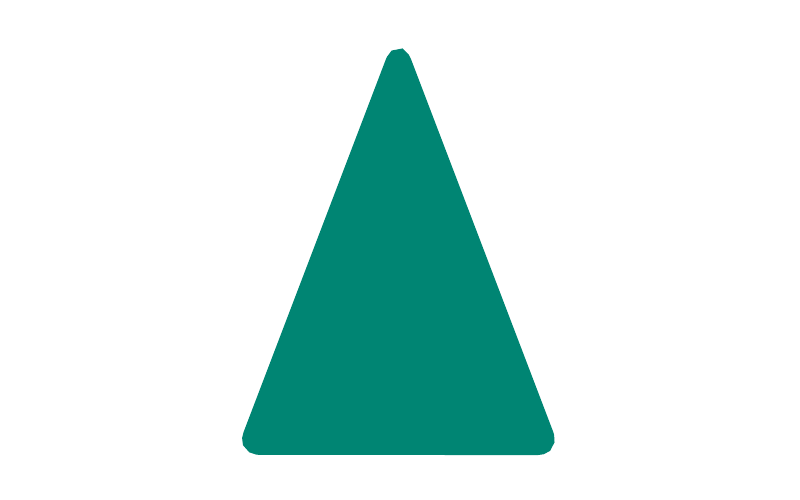
\includegraphics[height=1.5em]{figuras/neurônios/pca3.png}}}$ Piramidal do CA3 & Lamelar & 60 & 1.384 & 6.657 & 278.286 & 78.584 & 0.155 \\
$\vcenter{\hbox{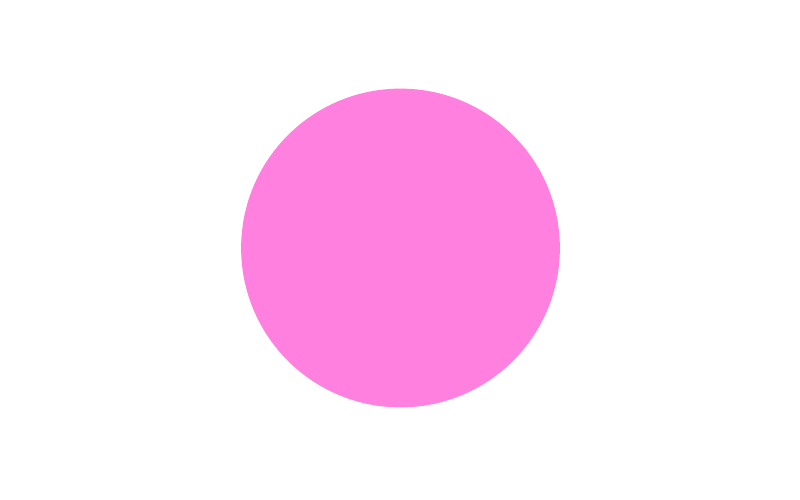
\includegraphics[height=1.5em]{figuras/neurônios/igc.png}}}$ Granular imatura & $\vcenter{\hbox{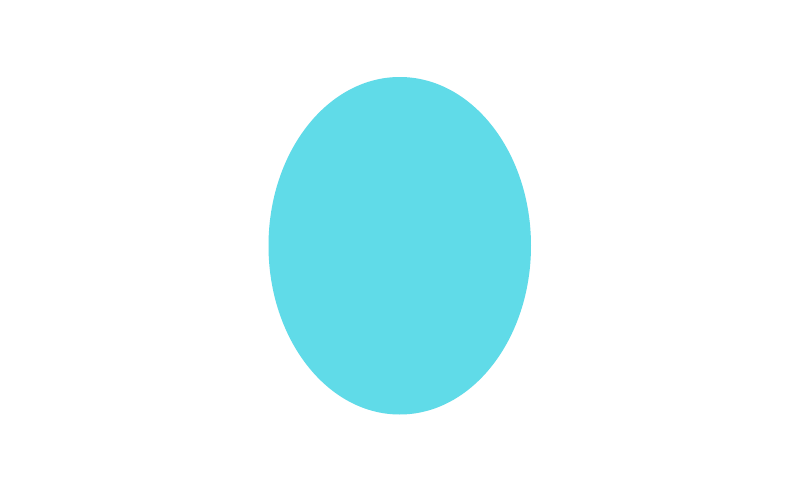
\includegraphics[height=1.5em]{figuras/neurônios/ica3.png}}}$ Inibitória do CA3 & Lamelar & 100 & 1.625 & 3.915 & 518.934 & 43.274 & 0.176 \\
$\vcenter{\hbox{
\includegraphics[height=1.5em]{figuras/neurônios/mc.png}}}$ Musgosa & $\vcenter{\hbox{\includegraphics[height=1.5em]{figuras/neurônios/mgc.png}}}$ Granular madura & Interlamelar & 0.2 & 2.394 & 5.357 & 166.162 & 20.224 & 0.304 \\
$\vcenter{\hbox{\includegraphics[height=1.5em]{figuras/neurônios/mc.png}}}$ Musgosa & $\vcenter{\hbox{\includegraphics[height=1.5em]{figuras/neurônios/igc.png}}}$ Granular imatura & Interlamelar & 0.2 & 2.394 & 5.357 & 166.162 & 20.224 & 0.304 \\
$\vcenter{\hbox{\includegraphics[height=1.5em]{figuras/neurônios/mc.png}}}$ Musgosa & $\vcenter{\hbox{\includegraphics[height=1.5em]{figuras/neurônios/hipp.png}}}$ HIPP & Interlamelar & 100 & 1.376 & 4.824 & 358.431 & 54.872 & 0.181 \\
$\vcenter{\hbox{\includegraphics[height=1.5em]{figuras/neurônios/mc.png}}}$ Musgosa & $\vcenter{\hbox{\includegraphics[height=1.5em]{figuras/neurônios/bc.png}}}$ Em cesto & Interlamelar & 100 & 1.996 & 3.396 & 117.365 & 69.316 & 0.255 \\
$\vcenter{\hbox{\includegraphics[height=1.5em]{figuras/neurônios/hipp.png}}}$ HIPP & $\vcenter{\hbox{\includegraphics[height=1.5em]{figuras/neurônios/mgc.png}}}$ Granular madura & Aleatória & 20 & 2.002 & 8.935 & 559.143 & 8.396 & 0.278 \\
$\vcenter{\hbox{\includegraphics[height=1.5em]{figuras/neurônios/hipp.png}}}$ HIPP & $\vcenter{\hbox{\includegraphics[height=1.5em]{figuras/neurônios/igc.png}}}$ Granular imatura & Aleatória & 10 & 2.002 & 8.935 & 559.143 & 8.396 & 0.278 \\
$\vcenter{\hbox{\includegraphics[height=1.5em]{figuras/neurônios/hipp.png}}}$ HIPP & $\vcenter{\hbox{\includegraphics[height=1.5em]{figuras/neurônios/bc.png}}}$ Em cesto & Aleatória & 2 & 1.709 & 5.982 & 367.198 & 15.292 & 0.221 \\
$\vcenter{\hbox{\includegraphics[height=1.5em]{figuras/neurônios/bc.png}}}$ Em cesto & $\vcenter{\hbox{\includegraphics[height=1.5em]{figuras/neurônios/mgc.png}}}$ Granular madura & Lamelar & 100 & 2.451 & 6.543 & 433.876 & 6.347 & 0.332 \\
$\vcenter{\hbox{\includegraphics[height=1.5em]{figuras/neurônios/bc.png}}}$ Em cesto & $\vcenter{\hbox{\includegraphics[height=1.5em]{figuras/neurônios/igc.png}}}$ Granular imatura & Lamelar & 100 & 2.451 & 6.543 & 433.876 & 6.347 & 0.332 \\
$\vcenter{\hbox{\includegraphics[height=1.5em]{figuras/neurônios/bc.png}}}$ Em cesto & $\vcenter{\hbox{\includegraphics[height=1.5em]{figuras/neurônios/hipp.png}}}$ HIPP & Aleatória & 2 & 1.408 & 6.544 & 534.182 & 8.385 & 0.24 \\
$\vcenter{\hbox{\includegraphics[height=1.5em]{figuras/neurônios/pca3.png}}}$ Piramidal do CA3 & $\vcenter{\hbox{\includegraphics[height=1.5em]{figuras/neurônios/pca3.png}}}$ Piramidal do CA3 & Aleatória & 2 & 0.603 & 9.516 & 278.258 & 27.513 & 0.172 \\
$\vcenter{\hbox{\includegraphics[height=1.5em]{figuras/neurônios/pca3.png}}}$ Piramidal do CA3 & $\vcenter{\hbox{\includegraphics[height=1.5em]{figuras/neurônios/mc.png}}}$ Musgosa & Lamelar & 10 & 2.035 & 4.297 & 359.116 & 40.457 & 0.236 \\
$\vcenter{\hbox{\includegraphics[height=1.5em]{figuras/neurônios/pca3.png}}}$ Piramidal do CA3 & $\vcenter{\hbox{\includegraphics[height=1.5em]{figuras/neurônios/ica3.png}}}$ Inibitória do CA3 & Aleatória & 100 & 1.247 & 4.525 & 525.605 & 23.321 & 0.189 \\
$\vcenter{\hbox{\includegraphics[height=1.5em]{figuras/neurônios/ica3.png}}}$ Inibitória do CA3 & $\vcenter{\hbox{\includegraphics[height=1.5em]{figuras/neurônios/pca3.png}}}$ Piramidal do CA3 & Aleatória & 100 & 1.462 & 7.793 & 416.282 & 20.63 & 0.203 \\
\bottomrule
\end{tabular}}
\caption{Parâmetros das sinapses entre as populações neuronais. Conexões aleatórias ocorrem entre todas as células
              de ambas as populações; conexões lamelares ocorrem entre células da mesma lamela; conexões interlamelares ocorrem
              entre as células de uma lamela com todas as demais. A probabilidade de conexão $P$ diz respeito à porcentagem de
              conexões entre as populações neuronais de acordo com a condição de conexão.}
\label{tab:synapse_params}
\end{table}



\section{Plasticidade de longo prazo}

A plasticidade de longo prazo será implementada exclusivamente nas sinapses recorrentes entre as células piramidais do CA3 (PCA3),
permitindo que a rede aprenda e armazene padrões de memória. O modelo de plasticidade será baseado no trabalho
de~\citeonline{kopsickFormation2024}, que utiliza uma regra de plasticidade dependente do tempo de disparo (STDP,
\textit{Spike-Timing-Dependent Plasticity}).

Especificamente, será empregada uma regra STDP simétrica e hebbiana, que promove o fortalecimento de sinapses entre neurônios que
disparam de forma temporalmente próxima, independentemente da ordem de disparo. Esta regra é descrita pela seguinte equação: 

\begin{equation}
    \label{eq:stdp}
    \Delta w = A e^{-|\Delta t|/\tau}
\end{equation}

Onde $\Delta w$ é a mudança no peso sináptico, $A$ é um parâmetro que determina a magnitude máxima da mudança no peso, $\tau$ é a
constante de tempo de decaimento da plasticidade e $\Delta t$ é a diferença temporal entre os disparos do neurônio pré e
pós-sináptico. Seguindo o modelo de~\cite{kopsickFormation2024}, a constante de tempo $\tau$ será definida como
\SI{20}{\milli\second}. O parâmetro $A$ será ajustado para modular a taxa de aprendizado da rede.

\begin{figure}[H]
    \centering
    \caption{Regra STDP simétrica e hebbiana com $A = 70$.}
    \includegraphics[width=0.5\textwidth]{figuras/symmetric_stdp}
    \label{fig:symmetric_stdp}
\end{figure}

Para evitar a saturação das sinapses, será empregada uma regra de renormalização dos pesos sinápticos
(Seção~\ref{sec:protocolo_treinamento_teste}) e um peso sináptico máximo de $w_{max}$ a ser definido experimentalmente.

\section{Neurogênese temporal}

Para investigar o impacto funcional da integração contínua de novos neurônios, será implementado um modelo de neurogênese
temporal. Este processo é fundamental para a manutenção de funções hipocampais como a aprendizagem e a memória ao longo do
tempo~\cite{aimoneRegulation2014, berdugo-vegaSharpening2023}. A simulação será dividida em duas fases principais. Na primeira
fase, a rede operará com sua configuração inicial, com $N_{mGC} = 1900$ e $N_{iGC} = 100$. Durante esta fase, a rede será exposta
a um conjunto de $N$ padrões de entrada, que serão aprendidos e armazenados nas sinapses recorrentes do CA3 através do mecanismo
de STDP.

Após a fase inicial de aprendizagem, as iGCs passarão por um processo de maturação simulada, transformando-se em mGCs. Esta
transição reflete as mudanças biológicas que ocorrem à medida que os novos neurônios se integram totalmente ao circuito do DG,
passando de um estado hiperexcitável para um estado maduro mais estável~\cite{abbottAdult2020}. A maturação será implementada
através da atualização dos seus parâmetros eletrofisiológicos e sinápticos para os valores correspondentes aos das mGCs
(Tabelas~\ref{tab:izhikevich_neuron_params} e~\ref{tab:synapse_params}). As conexões eferentes existentes, formadas durante a fase
imatura, serão preservadas. Adicionalmente, as células recém-maturadas passarão a ter sua conectividade aferente do EC aumentada
para o mesmo nível das mGCs, completando sua integração funcional no circuito.

Na segunda fase da simulação, após a maturação das primeiras iGCs, serão adicionadas mais 100 novas iGCs, simulando a contínua
integração de novos neurônios pela neurogênese adulta. Esse processo será repetido 3 vezes, tornando possível avaliar o desempenho
da rede gradativamente, com a maturação das iGCs. Serão implementados dois modelos de controle: um em que serão adicionadas sempre
mGCs na rede, sem as iGCs, e outro em que ao serem adicionadas as iGCs, haverá morte neuronal de número equivalente das mGCs. A
intenção desses modelos de controle é tornar possível avaliar apenas o papel da neurogênese adulta e das células imaturas geradas
por ela, comparando com os efeitos dos modelos de controle que também possuem aumento gradual de neurônios.


\section{Separação de padrões}\label{sec:separacao_padroes}

A metodologia para quantificar a separação de padrões foi baseada na utilizada por~\citeonline{kimEffect2024}. Para analisar a
separação de padrões em diferentes níveis de similaridade de padrões de entrada e o impacto da neurogênese adulta, foram testadas
11 versões diferentes do modelo: um controle sem neurogênese adulta ($N_{mGC} = 2000$) e outros 10 com neurogênese em diferentes
níveis de conectividade ($N_{mGC} = 1900$ e $N_{iGC} = 100$), conforme ilustra a Figura~\ref{fig:diagrama_entrada_saida}. O nível
de conectividade é dado em porcentagem, onde 100\% corresponde às iGCs possuindo a mesma probabilidade de conexão EC-GC que as
mGCs; a intenção é simular a não total integração das iGCs no circuito, com seus dendritos ainda não tão desenvolvidos. Para cada
modelo, são gerados 20 conjuntos de 10 padrões de entrada. Cada conjunto de padrões de entrada consiste de um padrão aleatório
original, gerado aleatoriamente, e 9 padrões similares a ele, de 90\% de similaridade a 10\%. Um padrão de entrada consiste em um
vetor binário de tamanho $N_{EC} = 400$, representando o estado de ativação de cada neurônio do EC, em que neurônios ativos
disparam de acordo com a distribuição de Poisson com uma frequência de \SI{40}{\hertz}. Todo padrão de entrada possui apenas 10\%
de neurônios ativos. Para gerar padrões com diferentes níveis de similaridade, uma fração aleatória de $X\%$ dos neurônios ativos
é mantida ativa, enquanto que os demais $(100 - X)\%$ são desativados e uma mesma quantia de neurônios inicialmente inativos, é
ativada, para manter o nível de atividade do padrão de 10\% (40 neurônios ativos).

Cada padrão é simulado por \SI{1500}{\milli\second} no tempo da simulação, sendo que os primeiros \SI{500}{\milli\second} são
ignorados enquanto a rede se estabiliza. O padrão de saída de uma população de neurônios, seja ela a população de mGCs, iGCs ou
PCA3s, consiste em um vetor binário com valor 1 para o índice do neurônio que disparou ao menos uma vez durante o intervalo de
\SI{1000}{\milli\second}.

\begin{figure}[H]
    \centering
    \caption{Diagrama do protocolo de geração e recordação dos padrões de entrada e saída. Cada um dos 11 modelos passa por 20
    conjuntos de 10 padrões de entrada, totalizando 200 simulações de \SI{1500}{\milli\second} cada. Os primeiros
    \SI{500}{\milli\second} são ignorados enquanto a rede se estabiliza. O padrão de saída, aqui ilustrado para a população de
    mGCs, consiste em um vetor binário com valor 1 para o índice do neurônio que disparou ao menos uma vez durante o intervalo de
    \SI{1000}{\milli\second}.}
    \includegraphics[width=\textwidth]{figuras/diagrama_entrada_saida}
    \label{fig:diagrama_entrada_saida}
\end{figure}

Para caracterizar a separação de padrões, é comparada a sobreposição entre os padrões de atividade neural na entrada (células do
córtex entorrinal) e na saída (células granulares do DG, ou piramidais do CA3) da rede. Um padrão é definido por um representação
binária de tamanho $N$, onde $N$ é o número total de neurônios de uma população específica, em que neurônios que dispararam ao
menos uma vez durante o intervalo de tempo da simulação são representados por 1 e os que não dispararam são representados por 0.
Para um par de padrões $A^{(l)}$ e $B^{(l)}$ (onde $l \in \{in, out\}$ para entrada e saída, respectivamente), a distância entre
os padrões $D_p^{(l)}$ é definida como:

\begin{equation}
    \label{eq:dp}
    D_p^{(l)} = \frac{O^{(l)}}{D_a^{(l)}}
\end{equation}

Nesta equação, $O^{(l)}$ representa o grau de ortogonalização e $D_a^{(l)}$ o grau médio de ativação dos dois padrões. O grau médio de ativação $D_a^{(l)}$ é a média aritmética dos graus de ativação de cada padrão, $A^{(l)}$ e $B^{(l)}$:

\begin{equation}
    \label{eq:da}
    D_a^{(l)} = \frac{D_a^{(A^{(l)})} + D_a^{(B^{(l)})}}{2}
\end{equation}

O grau de ativação de um padrão individual é a fração de neurônios ativos (representados por 1 em uma codificação binária) no padrão.
O grau de ortogonalização $O^{(l)}$, que mede a dissimilaridade entre os padrões, é calculado a partir do coeficiente de correlação de Pearson, $\rho^{(l)}$:

\begin{equation}
    \label{eq:o}
    O^{(l)} = \frac{1 - \rho^{(l)}}{2}
\end{equation}

Onde $\rho^{(l)}$ é o coeficiente de correlação de Pearson entre os padrões $A^{(l)}$ e $B^{(l)}$.
Considerando $\{a_i^{(l)}\}$ e $\{b_i^{(l)}\}$ ($i=1, \dots, N_l$) como as representações binárias do estado da $i$-ésima célula nos padrões $A^{(l)}$ e $B^{(l)}$ ($l \in \{in, out\}$), o coeficiente de correlação de Pearson é dado por:

\begin{equation}
    \label{eq:pearson}
    \rho^{(l)} = \frac{\sum_{i=1}^{N_l} \Delta a_i^{(l)} \cdot \Delta b_i^{(l)}}{\sqrt{\sum_{i=1}^{N_l} (\Delta a_i^{(l)})^2} \sqrt{\sum_{i=1}^{N_l} (\Delta b_i^{(l)})^2}}
\end{equation}

em que $\Delta a_i^{(l)} = a_i^{(l)} - \langle a^{(l)} \rangle$ e $\Delta b_i^{(l)} = b_i^{(l)} - \langle b^{(l)} \rangle$. A
notação $\langle \dots \rangle$ indica a média populacional sobre todas as células. O valor de $\rho^{(l)}$ varia entre -1 e 1,
portanto, $O^{(l)}$ varia entre 0 e 1 (Equação~\ref{eq:o}).

A partir das distâncias dos padrões de entrada ($D_p^{(in)}$) e saída ($D_p^{(out)}$), o grau de separação de padrões, $S_d$, é calculado como a razão entre elas:

\begin{equation}
    \label{eq:sd}
    S_d = \frac{D_p^{(out)}}{D_p^{(in)}}
\end{equation}

Um valor de $S_d > 1$ indica que os padrões de saída são mais distintos que os de entrada, caracterizando a separação de padrões. Inversamente, $S_d < 1$ indica uma convergência de padrões, onde os padrões de saída se tornam mais similares entre si.

\section{Auto-associação e completamento de padrões}

\subsection{Protocolo de treinamento e teste}\label{sec:protocolo_treinamento_teste}

O protocolo de treinamento e teste da rede para avaliar o armazenamento e a recuperação de padrões será baseado no método descrito
por~\cite{kopsickFormation2024}.

Na fase de treinamento, a rede será exposta a um conjunto de padrões de entrada distintos. Cada padrão consiste na ativação de uma
subpopulação específica de neurônios piramidais do CA3 através da injeção de corrente. Essa ativação induz um trem de disparos em
uma janela de tempo de \SI{20}{\milli\second}, correspondente a um ciclo gama. Os diferentes padrões serão apresentados em
sequência, separados por janelas de \SI{200}{\milli\second}, simulando um código neural teta-gama. Durante toda a fase de
treinamento, a plasticidade sináptica (STDP) estará habilitada, permitindo o fortalecimento das conexões entre os neurônios
codificantes do mesmo padrão, formando uma assembleia neuronal. Após um determinado número de apresentações de padrões a ser
definido experimentalmente, os pesos sinápticos entre os neurônios piramidais serão renormalizados, um processo que simula a
homeostase sináptica que ocorre durante o sono de ondas lentas, para evitar a saturação das sinapses e estabilizar os padrões
aprendidos~\cite{gonzalez-ruedaActivityDependent2018, kopsickFormation2024}.

Na fase de teste, a plasticidade sináptica será desabilitada para avaliar a capacidade da rede de recuperar os padrões memorizados
sem que haja modificações nas conexões. Serão apresentadas versões degradadas dos padrões originais, onde apenas uma fração dos
neurônios da assembleia correspondente é ativada. A resposta da rede será então analisada para verificar se a atividade das
conexões recorrentes é capaz de reconstruir o padrão completo, através do completamento de padrões.

\subsection{Quantificação}

A força da auto-associação, ou seja, a formação das assembleias, será medida através de duas características das sinapses entre os
neurônios piramidais. A primeira é a razão sinal-ruído (SNR) da auto-associação, definida como a média dos pesos sinápticos entre
neurônios da mesma assembleia dividida pela média dos pesos sinápticos entre neurônios de assembleias distintas. Um SNR elevado
indica uma forte distinção entre as conexões intra e inter-assembleias. A segunda métrica é a porcentagem de sinapses dentro de
uma assembleia que atingiu o peso máximo, o que serve como um indicador de saturação sináptica.

O completamento de padrões será avaliado através de uma métrica de precisão de reconstrução de padrão, baseada
em~\cite{kopsickFormation2024}. Esta métrica utiliza o coeficiente de correlação de Pearson (Equação~\ref{eq:pearson}) entre os
padrões de entrada ou saída durante a fase de treinamento e de teste. 

Primeiramente, calcula-se a correlação do padrão de entrada, $\rho^{(in)}$, que é a correlação entre o padrão completo do EC
apresentado durante a fase de treinamento e o padrão degradado, ou incompleto, apresentado durante a fase de teste. Em seguida,
calcula-se a correlação do padrão de saída, $\rho^{(out)}$, que corresponde à correlação entre a atividade neural das PCA3s em
resposta ao padrão de treinamento completo, durante a codificação da assembleia, e a atividade em resposta ao padrão de teste
degradado.

A precisão de reconstrução do padrão, $R_p$, é então calculada como:

\begin{equation}
    \label{eq:rp}
    R_p = \frac{\rho^{(out)} - \rho^{(in)}}{1 - \rho^{(in)}}
\end{equation}

Um valor de $R_p > 0$ indica que ocorreu o completamento do padrão, ou seja, a representação na saída tornou-se mais similar ao
padrão original do que a entrada degradada. Um valor de $R_p = 1$ representa uma reconstrução perfeita.
